\begin{figure}[htbp]
\centering
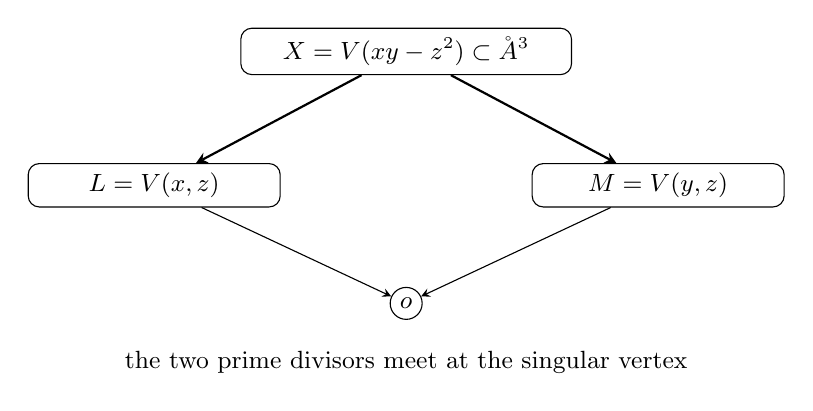
\begin{tikzpicture}[>=stealth,every node/.style={font=\small}]
\node[draw,rounded corners,align=center,minimum width=4.2cm] (x) at (0,1.7) {$X=V(xy-z^2)\subset\AA^3$};
\node[draw,rounded corners,align=center,minimum width=3.2cm] (l) at (-3.2,0) {$L=V(x,z)$};
\node[draw,rounded corners,align=center,minimum width=3.2cm] (m) at (3.2,0) {$M=V(y,z)$};
\node[draw,circle,inner sep=2pt] (o) at (0,-1.5) {$o$};
\draw[->,thick] (x)--(l);
\draw[->,thick] (x)--(m);
\draw[->] (l)--(o);
\draw[->] (m)--(o);
\node at (0,-2.25) {the two prime divisors meet at the singular vertex};
\end{tikzpicture}
\caption{The two distinguished ruling divisors on the quadric cone meet at the vertex.}
\label{fig:vi41-cone-divisors}
\end{figure}
